% !TEX encoding = UTF-8
% !TEX program = pdflatex
% !TEX root = relazione-MEMOC.tex
% !TeX spellcheck = it_IT

\section{Introduzione}

L'obiettivo della prima parte del progetto era quello di implementare un modello in CPLEX e di provarlo in modo da trovare la dimensione massima del problema che permette una risoluzione esatta entro un certo limite di tempo, mentre la seconda parte comprendeva l'implementazione di un algoritmo meta-euristico ad-hoc per il problema e di confrontarlo con CPLEX.

La sezione §\ref{sec:cplex} contiene la descrizione dell'implementazione del modello CPLEX con i relativi test, mentre la sezione §\ref{sec:genetico} contiene la descrizione dell'algoritmo genetico implementato e un confronto delle prestazioni rispetto a quelle ottenute da CPLEX.

\subsection{Generazione delle istanze}

Prima di implementare i vari algoritmi è stato necessario creare delle istanze per il problema.
\`E stato quindi creato uno script in Python in grado di generare delle istanze casuali a partire da un numero di nodi o fori.

Dato che il problema ha delle caratteristiche specifiche, ovvero visto che si tratta di schede perforate, è ragionevole assumere che i fori seguano un certo pattern.
Pertanto lo script è stato sviluppato in modo che possa generare anche delle istanze pseudo-casuali, ovvero delle istanze in cui ci sono blocchi di punti che compaiono vicini tra loro, raggruppati in rettangoli e a coppie.

In entrambi i casi, una volta generati i punti, le distanze sono state calcolate utilizzando la distanza euclidea.

\begin{figure}[htbp]
	\centering
	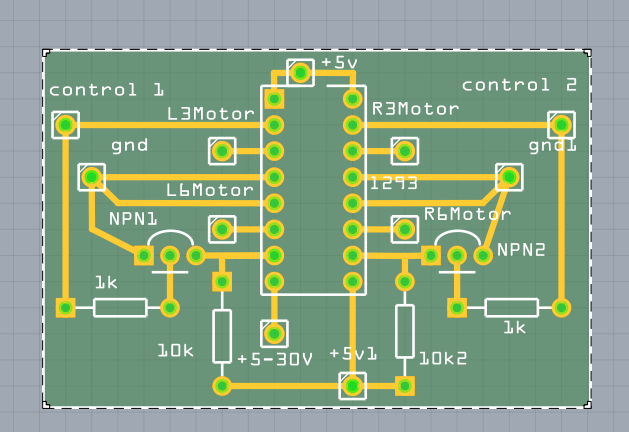
\includegraphics[width=.5\textwidth]{immagini/scheda.png}
	\caption{Esempio di scheda perforata presa come riferimento per la generazione delle istanze pseudo-casuali.}
\end{figure}